\documentclass[12pt, letterpaper, twoside]{article}
\usepackage[top=1.2in, bottom=1in, left=1in, right=1in]{geometry} %margins

\usepackage{xltxtra} %Xeletex Package
\usepackage{fontspec} %Font package
\usepackage{xunicode} %Xeletex
\usepackage{microtype} %better formatting

\usepackage[big,sf,bf]{titlesec} %set section title formats to big and a sans font

\usepackage{indentfirst} %indent first paragraphs always
\raggedbottom %keeps latex from stretching paragraphs apart if they do not fill the page

% **************** Colors ***************
\usepackage[usenames, dvipsnames]{color}
\definecolor{bg}{rgb}{0.95,0.95,0.95}

% **************** Spacing Command ***************
\usepackage{setspace}
\setstretch{2}

% **************** Language/Localization ***************
\usepackage[australian, spanish, american]{babel} %datetime incompatible with polyglossia
%\usepackage{polyglossia}
%\setdefaultlanguage[variant=american]{english}
%\setotherlanguage{spanish}

% *************** Set Fonts ***************
\defaultfontfeatures{Ligatures=TeX}
\setromanfont[Mapping=tex-text]{Baskerville}
\setsansfont[Mapping=tex-text]{Myriad Pro}
\newfontfamily\titleFont[Ligatures=TeX]{Myriad Pro}
\setmonofont{DejaVu Sans Mono}

% **************** Set Header/footer ***************
\usepackage{fancyhdr}
\fancyhf{} %reset header and footer
\fancyhf[HLE,HRO]{\thepage} %set page number, in header, changing sides odd (r) to even (l)
\fancyhf[HCE,HCO]{Keifer -- Thesis Proposal} %set center of header, odd and even
\renewcommand{\headrulewidth}{0pt} %remove horizontal rule at bottom of header

% *************** Set Date Format ***************
\usepackage[nodayofweek]{datetime}
%\setdefaultdate{\dateaustralian} %gets dates of dd month yyyy without ordinal or comma

% *************** Set Biblatex Style and Options ***************

\usepackage{csquotes}
\usepackage[authordate-trad, backend=biber, dateabbrev=true, firstinits=true, maxcitenames=3, isbn=false, doi=false, eprint=false, shorthandfull, sorting=nyt, sortcites=true, ibidtracker=false]{biblatex-chicago}
\addbibresource[datatype=bibtex]{thesis.bib}

%Check for page range in postnotes to use a colon not comma
\renewcommand{\postnotedelim}{\iffieldpages{postnote}{\addcolon\space}{\addcomma\space}} 
\DeclareFieldFormat{postnote}{#1} 

%Fix date format in bib -- could be moved to external .lbx file (with comments; change DefineBib... to DeclareBib...)
%%%%\DeclareLanguageMapping{american}{american-dmy}
%%%%
%%%%\begin{filecontents}{american-dmy.lbx}
%%%%\ProvidesFile{american-dmy.lbx}[american localisation with dmydate format for long dates]
%%%%
%%%%\InheritBibliographyExtras{american}
\DefineBibliographyExtras{american}{%
  \protected\def\mkbibdatelong#1#2#3{%
    \iffieldundef{#3}
      {}
      {\stripzeros{\thefield{#3}}%
       \iffieldundef{#2}{}{\nobreakspace}}%
    \iffieldundef{#2}
      {}
      {\mkbibmonth{\thefield{#2}}%
       \iffieldundef{#1}{}{\space}}%
    \iffieldbibstring{#1}{\bibstring{\thefield{#1}}}{\stripzeros{\thefield{#1}}}}%
}
%%%%\InheritBibliographyStrings{american}
%%%%\endinput
%%%%\end{filecontents}

% *************** Make ref links whole ref in text *****************
%%%%\DeclareCiteCommand{\cite}
%%%%  {\usebibmacro{prenote}}
%%%%  {\usebibmacro{citeindex}%
%%%%   \printtext[bibhyperref]{\usebibmacro{cite}}}
%%%%  {\multicitedelim}
%%%%  {\usebibmacro{postnote}}
%%%%
%%%%\DeclareCiteCommand*{\cite}
%%%%  {\usebibmacro{prenote}}
%%%%  {\usebibmacro{citeindex}%
%%%%   \printtext[bibhyperref]{\usebibmacro{citeyear}}}
%%%%  {\multicitedelim}
%%%%  {\usebibmacro{postnote}}
%%%%
%%%%\DeclareCiteCommand{\parencite}[\mkbibparens]
%%%%  {\usebibmacro{prenote}}
%%%%  {\usebibmacro{citeindex}%
%%%%    \printtext[bibhyperref]{\usebibmacro{cite}}}
%%%%  {\multicitedelim}
%%%%  {\usebibmacro{postnote}}
%%%%
%%%%\DeclareCiteCommand*{\parencite}[\mkbibparens]
%%%%  {\usebibmacro{prenote}}
%%%%  {\usebibmacro{citeindex}%
%%%%    \printtext[bibhyperref]{\usebibmacro{citeyear}}}
%%%%  {\multicitedelim}
%%%%  {\usebibmacro{postnote}}
%%%%
%%%%\DeclareCiteCommand{\footcite}[\mkbibfootnote]
%%%%  {\usebibmacro{prenote}}
%%%%  {\usebibmacro{citeindex}%
%%%%  \printtext[bibhyperref]{ \usebibmacro{cite}}}
%%%%  {\multicitedelim}
%%%%  {\usebibmacro{postnote}}
%%%%
%%%%\DeclareCiteCommand{\footcitetext}[\mkbibfootnotetext]
%%%%  {\usebibmacro{prenote}}
%%%%  {\usebibmacro{citeindex}%
%%%%   \printtext[bibhyperref]{\usebibmacro{cite}}}
%%%%  {\multicitedelim}
%%%%  {\usebibmacro{postnote}}
%%%%
%%%%\DeclareCiteCommand{\textcite}
%%%%  {\boolfalse{cbx:parens}}
%%%%  {\usebibmacro{citeindex}%
%%%%   \printtext[bibhyperref]{\usebibmacro{textcite}}}
%%%%  {\ifbool{cbx:parens}
%%%%     {\bibcloseparen\global\boolfalse{cbx:parens}}
%%%%     {}%
%%%%   \multicitedelim}
%%%%  {\usebibmacro{textcite:postnote}}
  
%Set custom strings for url and date labels (available at and last accessed)
\DefineBibliographyStrings{american}{%
  url = {available at},
  urlseen = {last accessed},
}
\DeclareFieldFormat{url}{\bibstring{url}\addcolon\space\url{#1}}
\DeclareFieldFormat{urldate}{\mkbibparens{\bibstring{urlseen}\addcolon\space{#1}}}

% Set url + date appearance in bib (add doi here if needed)
\renewbibmacro*{bib+doi+url}{%
  \usebibmacro{url+urldate}
  }
  
%Remove Quotes around titles
\DeclareFieldFormat
  [article,inbook,incollection,inproceedings,patent,thesis,unpublished]
  {title}{#1\isdot}
  
\appto{\bibsetup}{\raggedright} %align left to prevent stretched urls (perhaps remove?)

% /end bib settings

% **************** Blank Page Commmand ***************
\usepackage{afterpage}
\newcommand\blankpage{%
    \null
    \thispagestyle{empty}%
    %\addtocounter{page}{-1}%
    \newpage}
    
% ****************** Other packages ****************
\usepackage[small,compatibility=true]{caption} % can be 10pts, per thesis guidelines

\usepackage{varioref} %to include \vref s to important things on other pages
\usepackage{comment} %now can \begin and \end {comment}s
\usepackage{amssymb} %extra math symbols
\usepackage{amsmath} %extra math support
\usepackage{ifthen} %needed for some macros
\usepackage{multirow} %create tabular cells spanning multiple rows
%\usepackage{xspace} %Define commands that appear not to eat spaces
\usepackage{url} %for url support
\urlstyle{same} %set url font to main font
%\usepackage{makeidx} %use \makeindex to make an index
\usepackage{needspace}
\usepackage{booktabs} %table package
\usepackage{tabularx} %for stretchy tables
\usepackage{colortbl} %to allow color in tables
\usepackage{enumitem} %for lists
\usepackage[figuresright]{rotating} %use \begin{sidewaysfigure} or sidewaystable to rotate large floats 
%\usepackage{longtable} %if need to make tables longer than one page
\vrefwarning %warnings, not errors, for vrefs for varioref package

\usepackage{minted} %for code snippets; use \begin{minted}[mathescape, linenos, etc]{python}
\usemintedstyle{tango}

% ****************** For Figures and Graphics *******************
\usepackage{graphicx}
\usepackage[justification=centering, labelfont=bf]{caption} %caption package with centering
\usepackage{subcaption} %allows subfigure captions
\captionsetup[sub]{font=footnotesize} %The subcaption settings
\captionsetup{compatibility=false} %To make caption package work
%\usepackage{cleveref} %Use \cref to add prefix to refs (i.e. Fig., Table, etc.)
%\usepackage{flafter} %Don't place floats until after refs

%To define \captionabove command for tables
\makeatletter
\newcommand{\captionabove}[2][]{%
    \vskip-\abovecaptionskip
    \vskip+\belowcaptionskip
    \ifx\@nnil#1\@nnil
        \caption{#2}%
    \else
        \caption[#1]{#2}%
    \fi
    \vskip+\abovecaptionskip
    \vskip-\belowcaptionskip
}

% ****************** HREF *******************
%ALWAYS LOAD HYPERREF LAST!
%Hyperref package for links -- colors set here
\usepackage{hyperref}
\hypersetup{colorlinks,
%linkcolor=MidnightBlue,
%filecolor=ForestGreen,
%urlcolor=BrickRed,
%citecolor=MidnightBlue}
linkcolor=Black,
filecolor=Black,
urlcolor=Black,
citecolor=Black}

\newcommand{\thesisTitle}{Phenological classification of crops in Northwest Argentina using 250-meter MODIS imagery}
\newcommand{\thesisSubtitle}{A thesis proposal}
\newcommand{\thesisAuthor}{Jarrett A. Keifer}
\newcommand{\thesisDegree}{Master of Art}
\newcommand{\thesisDept}{Geography}
\newcommand{\thesisDate}{11 June 2014}
\newcommand{\thesisAbstract}{Subtropical deforestation in Latin America is thought to be driven by demand for agricultural land, particularly to grow soybeans. However, existing remote sensing methods that can differentiate crop types to verify this hypothesis require high spatial or spectral resolution data, or extensive ground truth information to develop training sites, none of which are freely available for much of the world. Here, I propose a new method of crop classification using multi-temporal MODIS vegetation indices as a base image from which to extract crops using their phenologies. I test and refine this method in Kansas, USA using the USDA crop data layer as reference. I then test the applicability of the method to other regions of the world by applying it to data from Pellegrini, Santiago Del Estero, Argentina. The study is to examine if using phenological profiles in image classification is a viable method to verify the initial hypothesis that soybeans are driving deforestation in subtropical South America.             The ability to map agricultural lands by crop type is crucial to understanding the geography and dynamics of land use and land cover change. Existing remote sensing methods that can differentiate crops by type require high spatial resolution data, high spectral resolution data, or extensive ground truth information to develop training sites, none of which are freely available for much of the world. As an alternative, I propose a new method of crop classification using multi-temporal MODIS vegetation indices as a base image from which to extract crops using their phenologies. I test and refine this method in Kansas, USA using the USDA Cropland Data Layer as reference. I discuss the numerous factors that effect the application and accuracy of the method, the method’s current limitations, and how the method might be further tested and refined.}

%% *************** Document style definitions ***************

% ******************************************************************
% This file defines the document design.
% Usually it is not necessary to edit this file, but you can change
% the design if you want.
% ******************************************************************

% The origin of this file is not clear.  Here is one copy:
% https://subversion.cs.uu.nl/repos/staff.doaitse.wxFlashkell/MasterThesis/style_old.tex
% Emerson Murphy-Hill (emerson@cs.pdx.edu) has modified it.
% Jarrett Keifer (jkeifer@pdx.edu) has also modified it greatly. It is now using AAG format for the references, suitable for all geography theses.


%************************* NOTES ON FORMATTING *************************

%Spacing:
%  Cannot use the setspace package with memoir class. However, memoir has its own spacing commands, and they are exactly the same, except use camel-casing:
%    \begin{Spacing}{1.5} or \DoubleSpacing or \OnehalfSpacing or \SingleSpacing


% *************** Load packages ***************
% *************** Colors ***************
\usepackage[usenames, dvipsnames]{color}
%\definecolor{bg}{rgb}{0.95,0.95,0.95} 


% **************** Syntax Highlighting ******************
\usepackage{minted} %for code snippets; use \begin{minted}[mathescape, linenos, etc]{python}
\usemintedstyle{tango}


% ****************** For Figures and Graphics *******************
\usepackage{graphicx}
\usepackage[justification=centering, labelfont=bf, small, compatibility=true]{caption} %caption package with centering, and can be 10pts, per thesis guidelines
\usepackage{subcaption} %allows subfigure captions
\captionsetup[sub]{font=footnotesize} %The subcaption settings
\captionsetup{compatibility=false} %To make caption package work
%\usepackage{cleveref} %Use \cref to add prefix to refs (i.e. Fig., Table, etc.)
%\usepackage{flafter} %Don't place floats until after refs

%To define \captionabove command for tables
\makeatletter
\newcommand{\captionabove}[2][]{%
    \vskip-\abovecaptionskip
    \vskip+\belowcaptionskip
    \ifx\@nnil#1\@nnil
        \caption{#2}%
    \else
        \caption[#1]{#2}%
    \fi
    \vskip+\abovecaptionskip
    \vskip-\belowcaptionskip
}


% ************** ALL OTHERS **************

\usepackage{varioref} 
\usepackage{times}
\usepackage{comment}
\usepackage{amssymb}
\usepackage{amsmath}
\usepackage{ifthen}
\usepackage{multirow}
\usepackage{xspace}
\usepackage{url}
\urlstyle{sf}
\usepackage{makeidx}
\usepackage{needspace}
\usepackage{tabularx}
\usepackage{colortbl}
\usepackage{enumitem}
\usepackage{afterpage}
\usepackage{longtable}
\usepackage{lscape}
\usepackage{ulem}
\usepackage{epsfig}
\usepackage{amsthm}
\usepackage{booktabs}
\usepackage{stmaryrd}
\usepackage[figuresright]{rotating}
\usepackage{xltxtra} %Xeletex Package
\usepackage{fontspec} %Font package
\usepackage{xunicode} %Xeletex

\normalem %normal emphasis for package ulem
\vrefwarning %warnings, not errors, for vrefs for varioref package

%TODO MOVE ALL GROUPS OF SETTINGS (I.E. TABLES & FIGURES, DOCUMENT LAYOUT, ETC. TO NEW TEX FILES INSIDE A SETTINGS FOLDER]


% *************** Enable index generation ***************
\makeindex


% **************** Language/Localization ***************
\usepackage[australian, spanish, american]{babel} %datetime incompatible with polyglossia
%\usepackage{polyglossia}
%\setdefaultlanguage[variant=american]{english}
%\setotherlanguage{spanish}


% *************** Set Date Format ***************
\usepackage[nodayofweek]{datetime}
%\setdefaultdate{\dateaustralian} %gets dates of dd month yyyy without ordinal or comma


% ********* Reference Settings **********
\input{bibsettings.tex}


% *************** Set Fonts ***************
\defaultfontfeatures{Ligatures=TeX}
\setromanfont[Mapping=tex-text]{Baskerville}
\setsansfont[Mapping=tex-text]{Myriad Pro}
\newfontfamily\titleFont[Ligatures=TeX]{Myriad Pro}
\setmonofont{DejaVu Sans Mono}


% *************** Page layout ***************
%\settypeblocksize{*}{32pc}{1.618}

\setlrmarginsandblock{1.5in}{1.0in}{*}  % Left and right margins
\setulmarginsandblock{1.5in}{1.0in}{*}  % Top and bottom margins
\checkandfixthelayout

\setheadfoot{\onelineskip}{2\onelineskip}
%\setheaderspaces{*}{2\onelineskip}{*}

\def\baselinestretch{2}  % double space for PSU

\checkandfixthelayout


% *************** Chapter and section style ***************
\makechapterstyle{mychapterstyle}{%
    \renewcommand{\chapnamefont}{\normalfont\sffamily\bfseries\large}%
    \renewcommand{\chapnumfont}{\normalfont\sffamily\bfseries\large}%
    \renewcommand{\chaptitlefont}{\normalfont\sffamily\bfseries\LARGE}%
    \renewcommand{\printchaptertitle}[1]{%
        \chaptitlefont{##1}
        }%
    \renewcommand{\printchapternum}{%
        \chapnumfont\thechapter%
        }%
       
}

\renewcommand*{\cftappendixname}{Appendix\space}

\chapterstyle{mychapterstyle}

\setsecheadstyle{\normalfont\sffamily\bfseries\large}
\setsubsecheadstyle{\normalfont\sffamily\bfseries}
\setsubsubsecheadstyle{\normalfont\sffamily\bfseries}
\setparaheadstyle{\normalfont\sffamily}

\nouppercaseheads  % prevents the headers from being uppercase
\makeevenhead{headings}{\normalfont\sffamily\mdseries\rightmark}{}{\normalfont\sffamily\mdseries\thepage}
\makeoddhead{headings}{\normalfont\sffamily\mdseries\rightmark}{}{\normalfont\sffamily\mdseries\thepage}

\aliaspagestyle{chapter}{empty}%this suppresses numbers on chapters


% *************** Table of contents style ***************
\settocdepth{subsubsection}

\setsecnumdepth{subsubsection}
\maxsecnumdepth{subsubsection}
\settocdepth{subsubsection}
\maxtocdepth{subsubsection}


% ********** Commands for epigraphs **********
\setlength{\epigraphwidth}{0.57\textwidth}
\setlength{\epigraphrule}{0pt}
\setlength{\beforeepigraphskip}{1\baselineskip}
\setlength{\afterepigraphskip}{2\baselineskip}

\newcommand{\epitext}{\sffamily\itshape}
\newcommand{\epiauthor}{\sffamily\scshape ---~}
\newcommand{\epititle}{\sffamily\itshape}
\newcommand{\epidate}{\sffamily\scshape}
\newcommand{\episkip}{\medskip}

\newcommand{\myepigraph}[4]{%
	\epigraph{\epitext #1\episkip}{\epiauthor #2\\\epititle #3 \epidate(#4)}\noindent}
	
	
% **************** Blank Page Commmand ***************
\usepackage{afterpage}
\newcommand\blankpage{%
    \null
    \thispagestyle{empty}%
    %\addtocounter{page}{-1}%
    \newpage}
    

% *************** DRAFT OPTIONS ****************
\usepackage{ifdraft}
%\ifdraft{<draft case>}{<final case>}
%\ifoptiondraft {⟨option draft given⟩} {⟨option draft not given⟩}
%\ifoptionfinal {⟨option final given⟩} {⟨option final not given⟩}

% *************** Enable hyperlinks in PDF documents ***************
\ifpdf
    \pdfcompresslevel=9
        \usepackage[plainpages=false,pdfpagelabels,bookmarksnumbered,%
        colorlinks=true,%
        linkcolor=sepia,%
        citecolor=sepia,%
        filecolor=maroon,%
        %pagecolor=red,%
        urlcolor=sepia,%
        pdftex,%
        unicode]{hyperref} 
    \pdfimageresolution=600
    \usepackage{thumbpdf} 
\else
    \usepackage{hyperref}
\fi
\usepackage[all]{hypcap}  % fixes problem when  you click on a link and go to caption, not figure or table itself

\usepackage{memhfixc}


% *************** End of document style definition ***************

\tolerance=1000 %sets whitespace tolerance level (adjusts hyphenation)

\begin{document}

% *************** Title Page ***************
\begin{titlepage}
\begin{center}

~\\
~\\

\thispagestyle{empty}

\titleFont\LARGE\thesisTitle

%~\\

%\Large\thesisSubtitle

~\\

\large~A thesis proposal by \thesisAuthor

\vfill

\today

\end{center}
\end{titlepage}

\newpage
\thispagestyle{empty}
\vspace*{1.25in}
\subsection*{Abstract}
\noindent\thesisAbstract
\newpage

% *************** Body ***************
\pagestyle{fancy} %to use fancy hdrs
\chapter{Introduction}
\label{intro}

Deforestation has long been a concern throughout tropical South America. However, this process of land use/land cover (LULC) change from forest to other uses has been increasingly recognized in subtropical South America as a significant source of environmental degradation. Understanding the complex dynamics of subtropical deforestation is crucial given the prominent role of forests in debates about climate change, conservation, and the protection of endangered species \autocites{geist2002proximate}{zak2004do-subtropical}{bonnie2000counting}{houghton1994the-worldwide}{sala2000global}.

Currently, many perceive growing demand for agricultural land---particularly land for soybeans---to be one of the greatest pressures on South American subtropical forests \autocites{pengue2005transgenic}{grau2005agriculture}{altieri2006gm-soybean:}. Remote sensing has given researchers a tool to classify land cover and measure deforestation. However, existing multi-spectral and multi-temporal image classification techniques require extensive ground truth information for the accurate classification of common crop types using widely-available remotely-sensed data. Therefore, getting a complete picture of the dynamics of deforestation, including an understanding of agricultural pressures on forests, requires rarely-available high spatial or high spectral resolution data \autocite{senay2000using} or expensive field time gathering training site data. The development of a tool that can efficiently and effectively extract crop types using widely-available imagery would be of value in investigations of LULC change in areas under rapid agricultural expansion.

The primary goal of this thesis is to develop and test a phenological classification toolset that can identify and extract crop types from a multi-date vegetation index sequence assembled using free and publicly-accessible data from the National Aeronautics and Space Administration’s (NASA) Moderate Resolution Imaging Spectroradiometer (MODIS) sensor. The toolset was tested using the U.S. Department of Agriculture's (USDA) Cropland Data Layer (CDL) from a test field in Kansas, USA. The CDL data provided delineation and crop identification of agricultural fields in the study area. Overlaid on the MODIS data, the CDL crop boundaries allowed the extraction of reference phenological signatures for various summer crops. Using the Kansas-derived reference signatures, imagery of the 2014 summer growing season in the Department of Pellegrini, Santiago del Estero, Argentina was then classified with the toolset. I further preformed a classification accuracy assessment to examine the toolset's applicability in subtropical South America.

The body of this thesis is broken into seven chapters. The \hyperref[intro]{first chapter} gives an overview and an introduction of the research. The \hyperref[background]{second chapter} provides background information on deforestation and soybean cultivation in Argentina. \hyperref[studyareas]{The third} introduces the two study areas where the processing methods, presented in \cref{methods}, are applied. \Cref{results} reviews the results of said methods, and \cref{discussion} is a discussion of their significance. \cref{conclusion} closes the thesis with some concluding remarks.

An additional five appendices contain supporting information. \Cref{appendix:fieldwork} is a reflection of my time in Argentina doing the fieldwork for this project. \Cref{appendix:tools} documents the toolset created to implement the processing methods of \cref{methods} and the development process. All the initial testing of the tools is reviewed in \cref{appendix:testing}. \Cref{appendix:future} contains a collection of ideas for future testing and research. Lastly, \cref{appendix:cdl} is a brief note about the CDL dataset.
\chapter{Background}
\section{Deforestation and the \textit{Ley de Bosques} (Forest Act) in Argentina}

The conversion of forestland to other uses has seriously impacted Argentina’s forests. In 1915 it was remarked that 30 percent of the country had forest cover, but in 2001 only 10 percent remained forested \autocite{secretaria-de-d2001primer}. Over the period 1998 to 2002, Argentina lost over 940,000 hectares of forest cover \autocite{secretaria-de-a2007informe}. The high rate of deforestation concerned policymakers, and Law 26.331, or the \textit{Ley de Bosques} (Forest Act), was voted into law in 2007 in an effort to preserve remaining native forests. Areas of native forest are defined to be those with forest cover of at least 20 percent native species, and that have trees of a minimum of 7 meters high. The law designates red, yellow, and green areas, each with different restrictions on clearing and use. Red is assigned to areas of “high conservation value,” yellow is for areas that must be managed sustainably, and green allows “partial or total use” \autocite[25]{gulezian2009environmental}. Each provincial government was responsible for determining how to classify their native forest area, and each enacted the \textit{Ley de Bosques} regulations under the \textit{Ordenamiento Territorial de los Bosques Nativos} (Land Management Order for Native Forests, OTBN).

As a part of Law 26.331, ongoing land cover studies are done to examine the effectiveness of the legislation. Between 2006 and the passing of the law, 573,296 hectares of native forest cover were lost. From the passing of the law in 2007 and the classification of the OTBN areas in 2009, a further 473,001 hectares were deforested. From the enacting of the OTBN (in 2009) and 2011, some 459,108 hectares were found to have been lost \autocite{secreteria-de-a2012monitoreo}. The continued deforestation suggests that, in the context of the native forest areas, the \textit{Ley de Bosques} may have had a small effect in reducing deforestation, but overall levels still remain quite high. Consequently, some have begun to question the effectiveness of the law at slowing cutting \autocites{valpreda2012the-protection}{greenpeace-arge2013ley-de-bosques:}. Clearly, a better understanding of the driving forces of deforestation in Argentina needs to be developed.

\section{Soy and its effects}

The increase of soybean in Argentina has occurred at a rapid pace throughout the last two decades, making it the third largest producer of soy in the world \autocite{us-foreign-agri2013world}. Necessarily, as soy production rises, so does its spatial extent and the intensity of cultivation methods. Currently, almost all of Argentina’s soy production is using genetically modified (GM) varieties, specifically Monsanto’s “Roundup Ready” beans \autocite{greenpeace-inte2005the-expanding}. The highly mechanized and input intensive nature of this crop type calls into question other environmental consequences of soybean cultivation, such as pesticide runoff, glyphosate-resistant weeds, and soil depletion \autocite{pengue2005transgenic}.

A number of studies have addressed soy and deforestation in Northwest Argentina, but only one has used methods capable of mapping crop types in deforested areas \autocite{volante2005analisis}. However, this study by the Argentine \textit{Instituto Nacional de Tecnología Agropecuraia} (National Institute of Agricultural Technology, INTA) does not have well-documented methodology and has not been updated since 2005. Of the remainder, all used remote sensing techniques to classify only LULC and not specific crop types, leaving the effect of soy on LULC as an underlying assumption \autocites{grau2005agriculture}
{grau2008balancing}{grau2005globalization}
{boletta2006assessing}{gasparri2009deforestation}. While the extreme deforestation in Argentina is undeniable---and certainly soy plays a part---its role has not been examined in full, leaving unsubstantiated the perception of soy as the driving force in this process.

The goal of this research is to develop an image classification capable of mapping agricultural crops by type, allowing soy to be explicitly identified on remotely sensed imagery. The accurate and efficient mapping of soy distributions and their changes over time could allow further investigation of the roles of soy in deforestation. The direct and indirect effects soy crops have had on deforestation can thus be understood conceptually and systemically at both regional and local scales, which could lead to the development of more effective policies for land management \autocite{brown2007multitemporal}.

\chapter{Study Areas}
\label{chapter:studyareas}

This study used agricultural areas in Kansas, USA for testing and verification of the phenological classification method and applied the classification method to Pellegrini, Santiago del Estero, Argentina to test its effectiveness in subtropical South America.


\section{Kansas, USA}
\label{chapter:studyareas:kansas}

The state of Kansas is one of the big agricultural producers of the U.S. As one of the plains states, it is relatively flat across much of its extent, making it well suited to large highly-mechanized agro-industrial operations. In 2012, the three most extensive crops in the state were wheat, corn, and soybeans (\autoref{table:kansas}), which are also the most abundant crops in Pellegrini, Argentina. Additionally, Kansas has been the focus of a number of previous studies into the use of MODIS time-series for crop classification \autocites{wardlow2002discriminating}{wardlow2005state-level}{wardlow2007analysis}{wardlow2008large-area}, and has a very detailed and easily-accessible crop cover dataset in the form of the USDA CDL, making it a natural choice for a preliminary study area to test my method.

I have chosen a small 100 MODIS pixel by 100 MODIS pixel study area just northwest of Wichita, Kansas, which includes the communities of Valley Center, Sedgwick, and Halstead running roughly in a line from the southeast corner to the northwest corner (\autoref{fig:KSstudysite}. This is the area where I did testing and verification of the method (see \autoref{appendix:testing} for a full overview of the Kansas testing), and where I extracted the crop reference signatures used for the Argentina classification. The typical planting dates for a variety of crops in this region are shown in \autoref{table:KSplantingdates}. This specific study site was chosen due to the good mix of land covers including, but not limited to, corn, soy, sorghum, winter wheat, winter wheat and soy double crop, urban development, grassland, and forest in the CDL reference.


\begin{sstable}
  \centering
  \caption[Most extensive crops in Kansas, 2012.]{Most extensive crops in Kansas, 2012\\~\autocite[adapted from][]{usda2013kansascrops}.}
  \label{table:kansas}
  \begin{tabu}{lcc}
    \toprule
    \textbf{Crop} & \textbf{Acreage (1,000 acres)} & \textbf{Production (1,000 units)} \\
    \midrule
    Wheat & 9,100 & 382,200 \\
    Corn & 3,950 & 379,200 \\
    Soy & 3,810 & 83,820 \\
    All Hay & 2,750 & 4,340 \\
    All Forage & 2,750 & 4,545 \\
    Sorghum & 2,100 & 81,900 \\      
    \bottomrule
  \end{tabu}
\end{sstable}

\begin{ssfigure}
  \centering
  \includegraphics[width=\textwidth]{Graphics/KSstudysite.pdf}
  \caption{Kansas Study Site}
  \label{fig:KSstudysite}
\end{ssfigure}

\begin{ssfigure}
  \centering
  \includegraphics[width=\textwidth]{Graphics/KScdl.pdf}
  \caption{2012 Kansas Study Site Crop Cover}
  \label{fig:KScdl}
\end{ssfigure}

\begin{sstable}
  \centering
  \caption[Kansas Study Site Planting Dates]{Kansas Study Site Planting Dates\\~\autocite[adapted from][]{shroyer1996kansas}.}
  \label{table:KSplantingdates}
  \begin{tabu} to 4.5in {X[1,m,c]X[2,m,c]}
    \toprule
    \textbf{Crop} & \textbf{Planting Date Range} \\
    \midrule
    Wheat & \datenoyear{25}{9} to \datenoyear{20}{10} \\
    Triticale & \datenoyear{1}{9} to \datenoyear{25}{9} \\
    Winter Barley & \datenoyear{15}{9} to \datenoyear{10}{10} \\
    Spring Barley & \datenoyear{25}{2} to \datenoyear{15}{3} \\
    Spring Wheat & \datenoyear{25}{2} to \datenoyear{15}{3}\\
    Spring Oats & \datenoyear{25}{2} to \datenoyear{15}{3}\\
    Corn & \datenoyear{1}{4} to \datenoyear{10}{5} \\
    Sorghum & \datenoyear{15}{5} to \datenoyear{20}{6} \\
    Soybeans & \datenoyear{5}{5} to \datenoyear{10}{6} \\
    \bottomrule
  \end{tabu}
\end{sstable}


\section{Pellegrini, Santiago del Estero, Argentina}
\label{chapter:studyareas:pellegrini}

Santiago del Estero, a province in Northwest Argentina, has an area of 136,351 square kilometers, about the same as Arkansas, but a population of about 874,000 \autocite{estadistica-y-c2010a}. The entire province is classified within the \textit{Parque Chaqueño} (Chaco forest), but, like the rest of Argentina forests, the forested area has declined rapidly over the past fifteen years. During the period 1998 to 2002, 306,055 hectares were deforested \autocite{secretaria-de-a2007informe}. From 2006 through 2011, a further 701,030 hectares of forest were lost, 283,669 of which were after the enacting of the OTBN \autocite{secreteria-de-a2012monitoreo}. Over both of these time periods Santiago del Estero experienced the highest levels of deforestation in all of Argentina.

The Department of Pellegrini is an administrative area in the Northwest corner of the province of Santiago del Estero (\autoref{map:argentinaOverview}).\footnote{The Pellegrini boundary shapefile I obtained does not accurately reflect the bounds of the department on the ground. Particularly along the lengthy and straight northwestern edge, careful inspection reveals a lack of registration between the vector geometry and the obvious boundary visible in the background image. When investigating some of my sample points along the northern and southern edges, I got strange looks and comments about how this or that field was not within Pellegrini, my supposed study area. I want to acknowledge that I realize my study area is not actually the Department of Pellegrini proper, but an inaccurate representation as defined by a shapefile from the Internet. I use this inaccurate representation to ensure consistency, to allow repeatability, and to simplify spatial analysis.} The department has an area of 6,944 square kilometers, a size slightly larger than the state of Delaware, and a 2010 population of only 20,514 \autocite{estadistica-y-c2010b}. The primary municipality of the department is Nueva Esperanza, with a population of about 4,500. The frontier nature of Pellegrini seems to have limited deforestation in the department for some time, but the push for land has increased the rate of deforestation. Over the years 2001 to 2005, only 5,968 hectares were found to be deforested (Volante 2005). From 2006 to 2011 the area deforested increased to 75,349 hectares, some 39,480 hectares cut after the enacting of the OTBN, a rate much higher than previously witnessed \autocite{secreteria-de-a2012monitoreo}. Of the area cleared post-OTBN, 2,181 hectares were in red areas, the highest clearing of that designation in the nation. The vast majority of clearing, however, was 29,796 hectares in yellow areas. While Pellegrini’s total deforestation during the period 2006 to 2011 was not the highest in Santiago del Estero, as both Moreno Department and Alberdi Department had higher total deforestation, as a percent of total land area Pellegrini’s deforestation occurred at a greater rate: 10.85 percent of Pellegrini’s land area was cleared versus 10.45 percent and 7.91 percent of Moreno and Alberdi, respectively.

\textcite{volante2005analisis} found Pellegrini's primary summer crop over the years 2000 to 2005 to be soy, averaging about 40,000 hectares cultivated per year. Corn was the second most frequent crop, occupying about 7,500 hectares per year. \textit{Poroto}, a generic term for many types of common beans, were the third most popular, averaging a total cultivation of about 2,500 hectares per year. The primary winter crop was wheat, though cultivation varied wildly from less than 10,000 hectares in 2002 to over 31,000 hectares in 2004.

Specific planting dates for Pellegrini are not available, but crop calendars for Argentina as a while do provide generalized information \autocites{agriculture-for2008foreign}{sacks2010crop}{soybean-and-cor2013argentina}. Corn is typically planted mid-September through the end of November, and sorghum follows about twenty days later. Soybeans are planted in two groups: early and late. Early soy is often planted mid-November through the end of December, while late soy follows the harvesting of winter wheat, typically between the beginning of December through the middle of January. Compared to \autoref{table:KSplantingdates}, these dates are approximately six months offset, congruent with Argentina's opposing location in the Southern Hemisphere. However, the Argentina planting date ranges are noticeably longer than those in Kansas.

%Harvesting of both corn and sorghum occurs from the end of March through the middle of June. Early soy is harvested from the end of March through the middle of May while late soy is not ready until the end of April, taking until mid-June to be completely harvested.

\begin{ssfigure}
  \centering
  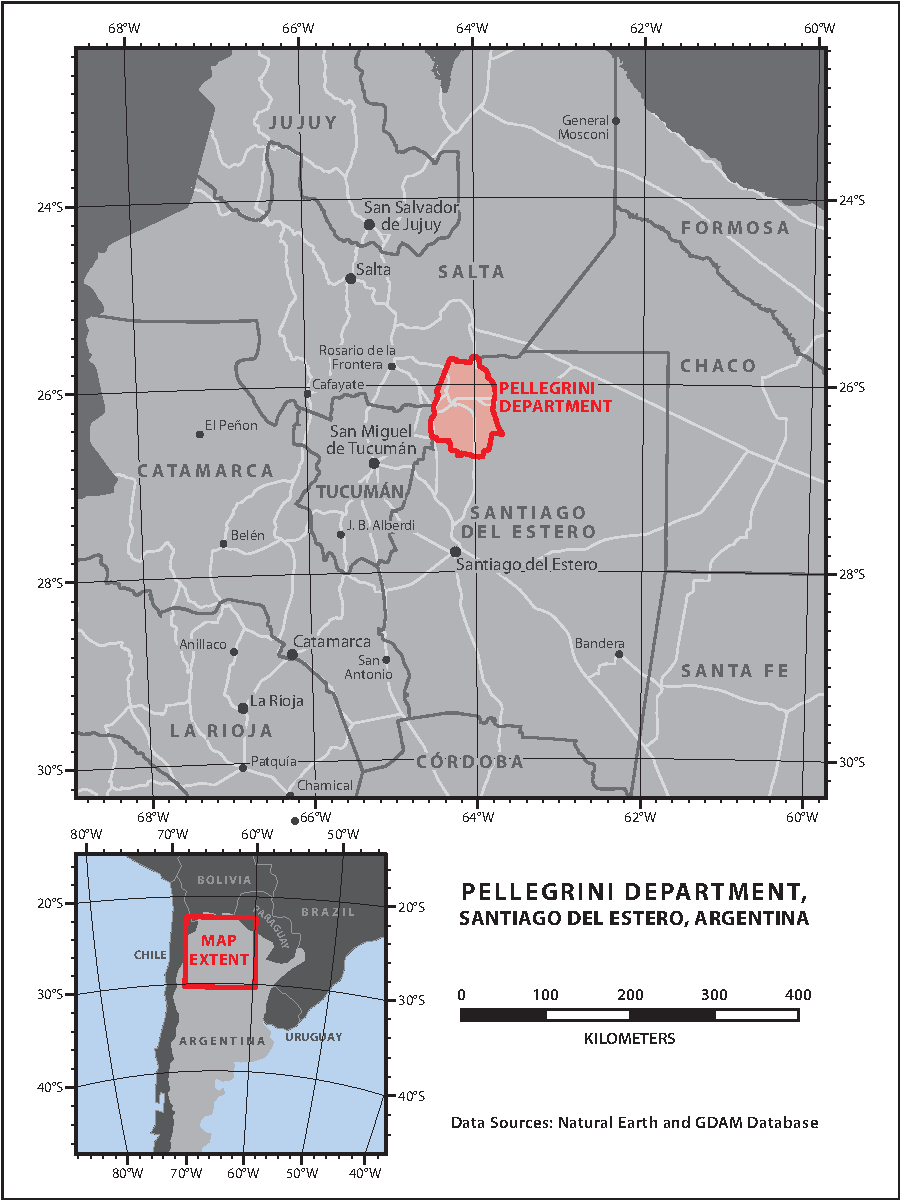
\includegraphics[width=\textwidth]{Graphics/argentinaOverview.pdf}
  \caption{The Department of Pellegrini and the Greater Northwest of Argentina}
  \label{map:argentinaOverview}
\end{ssfigure}

\begin{ssfigure}
  \centering
  \includegraphics[scale=.95]{Graphics/pellegrini75to14.pdf}
  \caption{Land Cover Change in Pellegrini from 1973 to 2014}
  \label{map:pellegriniCoverChange}
  \medskip
  \small
  These images show the progression of deforestation in Pellegrini. The lack of deforestation in the 1973-1975 composite is striking. As early as 1993, deforestation is visible, primarily in the Southwest along the RN34 highway. Little changed between 1993 and 2001, but by 2014 much more deforestation is visible throughout the entire area.\end{ssfigure}


\chapter{Data and Methods}
\label{chapter:methods}

\section{Overview}

The purpose of this study is to develop a set of tools to allow the classification of agricultural crops using a time series of imagery and known crop reference signatures and test the portability of the reference signatures. The data used for this study consists of the following:

\begin{Spacing}{1.2}
\begin{itemize}
  \item 250-meter MODIS 16-day Composite Vegetation Index images
  \item 30-meter 2012 USDA Cropland Data Layer (CDL): agricultural land cover raster dataset
  \item 30-meter Landsat 8 Operational Land Imager satellite imagery
  \item Shapefile of the administrative boundary of the Department of Pellegrini
  \item 2014 Land cover vector dataset with crop identifications for Pellegrini
\end{itemize}
\end{Spacing}

The first three datasets are publicly available from U.S. agencies. The Pellegrini boundary is from the GDAM Global Administrative Areas Dataset, version 1.0 (available at http://www.gdam.org). The land cover dataset for Pellegrini was digitized from Landsat 8 images (path 230, row 78), and the crop identifications were collected in the field.

An outline of the processing workflow is below:

\begin{Spacing}{1.2}
\begin{enumerate}
  \item Reproject the MODIS composite imagery
  \item Assemble individual composite images into single time series images, one for Kansas and one for Argentina
  \item Create a mask of all pure pixels (e.g. non-mixel) in the time series images
  \item Use the CDL to isolate the pure corn, soy, and sorghum pixels in the Kansas time series image.
  \item Identify the unique groups in each set of isolated pixels using k-means clustering
  \item Extract the pixel values for each cluster from the time series image and find the mean value for each date to find the unique signatures for each crop
  \item Validate the signatures by fitting the signatures to the time series image, then classifying the fit rasters to check the accuracy
  \item Fit the signatures to the Argentina time series image
  \item Classify the Argentina fit rasters and assess the accuracy
\end{enumerate}
\end{Spacing}

This chapter is a look at the theory and concepts behind this classification approach, the methods and fieldwork used to create the validation land cover dataset of Pellegrini, and the data processing steps used to generate the study results. Details about the specific tools in the classification toolset and the development process can be found in Appendix \ref{appendix:tools}. For a detailed explanation of all the testing proceeding this study, please see Appendix \ref{appendix:testing}. A thorough recounting of my field experience can be found in Appendix \ref{appendix:fieldwork}.


\section{Field Methods and Data Collection in Pellegrini}

While ground truth data was easily available for the Kansas study site, getting a ground truth dataset for verification of the classification in Pellegrini was not so simple. Such a dataset did not exist, necessitating onsite data collection. I visited Argentina mid-March to early April 2014 to gather field observations of summer crop types and to talk to local farmers about typical agricultural practices, summer and winter crop varieties, and planting and harvesting dates.

To guide my ground truth collection, I generated 400 random points inside the Pellegrini shapefile boundary, and used a Landsat OLI image as a reference for land cover (image date \formatdate{5}{2}{2014}). Where a point fell within a mixel, I allowed it to be moved within a 3-by-3 pixel window centered on the point's original pixel, trying as much as possible to keep the point within a pixel belonging to the feature type on which it originally fell. In certain limited cases, if a point fell quite obviously within a field but the center pixel and eight surrounding pixels were mixels and/or were not within the field, I allowed the point to be moved to the closest full pixel of that same continuous field. Of the 400 points, I had move 106 within the 3-by-3 window, and ten to a non-neighboring pixel within the same field.

The primary means of gathering the crop identities to complete the ground truth was direct observation. However, this strategy proved to be difficult in many cases; often, fields were not accessible due to road conditions or locked gated. Data not from direct observations came from interviews with farmers and land owners. In such cases, the interviewees were asked to identify their fields on printed maps with the reference Landsat imagery and describe their cultivars. The data from observations and interviews was recorded directly on the maps and later manually digitized.

Ancillary information about agricultural practices in the region was also collected whenever possible. It was a key goal to identify each crop's date range for planting and harvesting in order to allow the proper selection of MODIS imagery dates and setting of the $tshift$ bounds for Equation \ref{eq:gofx}.

\section{Data Processing}

\subsection{Resampling the CDL}

To use the CDL as a ground truth with the Kansas TSI, the 30-meter CDL pixels were resampled by majority to match the larger TSI pixels. This allowed a direct comparison between the crop values from the CDL and the pixel signatures in the TSI.

\subsection{Building the TSIs}

For this study, I chose to classify the 2012 Kansas summer growing season and the 2014 Argentina summer growing season. I assembled the MODIS 16-day composite VI images into multi-date time-series images (TSI) covering the growth cycle of the summer crops, where each band in a TSI is a 16-day composite VI and the bands are ordered consecutively (see Appendix \ref{appendix:tools:build} for the description of the Build Multidate Image Tools). The Kansas summer TSI covered the date range DOY 97 through DOY 273, and was made with data from the Terra satellite (LPDAAC product MOD13Q1, tile h10v05). Prior to creating the TSIs, each of the 16-day composites was reprojected from the native MODIS sinusoidal reference system using LPDAAC's MODIS Reprojection Tool \autocite{modis4.1}. I reprojected the Kansas data into the Albers Equal Area Conic projection for the contiguous USA using the 1983 North American Datum (WKID: 5070) to match the reference system of the USDA CDL.

In Argentina, as it is in the Southern Hemisphere and the seasons are inverted to those of the Northern hemisphere, the growing season shifts, as must the date range for the VI time-series. The TSI for Pellegrini must begin at the end of the proceeding year to adequately capture the entirety of the summer phenologies. To accomplish this, the time-series image for summer 2014 began with the 16-day composite image from DOY 353 of 2013 (or DOY −13 with reference to 2014) and ended with the image from DOY 161 of 2014 (MODIS grid tile h12v11). This specific date range was chosen based on information provided by local farmers to ensure coverage of the earliest planting and latest harvesting dates, as well as manual inspection of pixel signatures throughout the study area. Persistent clouds necessitated using an image from the Aqua satellite of DOY 105 (LPDAAC product MYD13Q1) in place of DOY 113 from Terra. Due to no viable imagery from Aqua or Terra, DOY 129 was interpolated via a simple mean from the DOY 105 Aqua image and the DOY 145 Terra image. The Argentina composite images were reprojected with the UTM Zone 20S reference system (WKID: 32720).

\subsection{Eliminating Mixels}

After building the TSIs, the next processing step was to eliminate mixels from the TSIs, to prevent errors caused by mixed temporal signatures (see Appendix \ref{appendix:testing:r2} for more information). Pure pixels, the non-mixels in an image, were isolated by intersecting the ground truth datasets with a vector grid of the TSI pixels. Then, all pixels with an area greater than an area threshold were selected as pure. Only these pure pixels were classified; the mixels in the TSIs were excluded.

The original 30-meter CDL raster served as the reference for finding the pure pixels in the Kansas study site. The raster was converted to vector polygons and intersected with the TSI grid polygons. From the resulting geometry, all polygons greater than 53,000 square meters (or 98 percent of a full MODIS pixel) were selected as pure. I also manually selected two sorghum pixel features that were omitted due to intermixed soy pixels. I chose to add these pixels due to the low number of sorghum features retained, and that the intermixed soy appeared to be errors.

For the Argentina analysis, the digitized features of identified fields were combined with manually digitized features of all large forested areas, unknown fields, and ``other'' areas. Some places where the land cover was mixed and could not be visually differentiated were not digitized and were considered to be composed entirely of mixels. The complete dataset of land cover was then intersected with the Argentina TSI grid. Through trial and error, a minimum area of 50,000 square meters was chosen as the threshold for pure pixels in the image.

\subsection{Extracting the Reference Temporal Signatures}

As a reference library of temporal signatures does not yet exist, I had to extract my own signatures from the Kansas TSI. To do so, the pure TSI pixels of each key summer crop---corn, soy, and sorghum---as specified in the resampled CDL were isolated in separate rasters. Each of separated rasters was clustered into three clusters using the ENVI \autocite{envi5.0} k-means tool with a 1.0 percent change threshold over 100 maximum iterations. The TSI pixels in each cluster were then sampled and averaged to find the three primary signatures for each crop\footnote{Given the existing literature about phenological classification, I do not believe crops have multiple signatures. I believe every crop as a theoretical ideal signature, which can be made to fit any actual signature using the $xscale$, $yscale$, and $tshift$ transformations in Equation \ref{eq:gofx}, barring any unusual effects of weather or other forces impacting crop development (a mid-season drought, for example, may cause a crop signature with double peaks due to the partial dying off and regeneration of the plants). However, given my choice of the CDL as my source of ground truth, I have had to make the assumption that it is highly accurate, despite any evidence to the contrary (see my discussion of the CDL beginning in \autoref{appendix:testing:r3}). Therefore, I use the clustering to derive the signatures that will create a classification most comparable to the CDL.} (see \autoref{appendix:tools:extract} for information about the Extract Signatures Tool).

\subsection{Fitting the Reference Signatures to the TSIs}

\autoref{eq:1} (page \pageref{eq:1}) was implemented using the programming language Python \autocite{python2.7.8} with a command line interface to allow easy processing of the TSIs. Details of the tool can be found in \autoref{appendix:tools:fit} on page \pageref{appendix:tools:fit}. The tool iterates through every pixel in a TSI, comparing each reference signature with the pixel signature. The tool is able clip an input TSI to either pixel bounds or a shapefile containing a polygon, and can also use an optional point shapefile to limit the processed pixels to only those coincident with points. An output raster is created for each signature to record the RMSE from every pixel comparison.

The reference signatures extracted from the Kansas TSI clusters were fit to the Kansas TSI to verify the classifier. The TSI was clipped to pixel row 2482 and column 1089, extending 100 rows and 100 columns. Then, the same Kansas signatures were fit to the Pellegrini TSI, which was clipped to the boundary shapefile. The fit rasters from each TSI were then classified. In both cases, the bounds for the $xscale$ and $yscale$ parameters were 0.6 to 1.4. The $tshift$ bounds for the Kansas processing were -10 to +10 days, while the bounds for the Pellegrini processing were 120 to 140 days (still $\pm10$ days, but shifted 130 days).\footnote{I have not formally tested other bounds. See Appendix \ref{appendix:future:fitting}.}

\subsection{Classifying the Fit Rasters}

The classification process is complex; Appendix \ref{appendix:tools:classify} contains a full discussion of the process, so I will refrain from a lengthy description here.

Classifying the fit rasters first requires thresholding the values in each raster, then finding the lowest value for each pixel. The signature with the lowest thresholded fit value has the best fit, and the pixel is classified as that crop. The thresholding prevents pixels with poor fit values from being classified as a crop. If a pixel has no remaining fit values after thresholding, it is classified as ``other.'' Currently, appropriate threshold values are not well understood, so to find the best classification, the classification tool must brute-force through many combinations of thresholds within a user-specified range, classifying the fit rasters, and calculating the accuracy of each threshold combination in comparison with the ground truth dataset. A raster of the classification with the best accuracy is retained.

For the Kansas classification, it was easy to try iterating through different threshold ranges. However, the Argentina classification was not as straightforward. As the tool must brute-force through every threshold combination, the time required to find the best threshold in a range is exponential, given by the number of threshold steps to the power of the number of images, times the number of seconds for each iteration. The Kansas classification took under 0.3 seconds per iteration; classifying the larger area of Pellegrini took substantially more time, somewhere between three and four seconds per iteration. The increased processing time ruled out using more than two or three steps in any given iteration. Consequently, in the case of the Argentina classification, I found it much more efficient to iterate through a range of threshold values using a single threshold value across all the fit rasters, then manually refine the thresholds until a suitable threshold combination was found.
\chapter{Timeline}

I hope to have finished the classification algorithm by the beginning of winter term 2014.  At that point, I will run the testing on the Kansas sample areas to find the best reference curves. Once that testing is completed, I will use those curves to classify MODIS data of Pellegrini from the 2012 -- 2013 growing season. This will provide me with a rough picture of the crop cover my method will find for 2013 -- 2014, and from this I can use a stratified random sampling technique to better ensure my ground truthing will contain sufficient sample points in each land cover class. In March 2014 I plan to do fieldwork in Pellegrini to collect the ground truth data for these points. I have chosen the month of March specifically because it is in the middle of the summer growing season, and I can get ground truth data for summer crop identification as the crops are growing. Winter crops, such as winter wheat, will need to be verified by inquiring with field owners, or confirmed by visual interpretation of Landsat imagery. In spring term 2014, I will classify 2013 -- 2014 data for Pellegrini, calculate the accuracy using the ground truth acquired in March, and begin writing. I plan to finish my work and writing over summer 2014 and present fall 2014.

\chapter{Results}
\section*{Preliminary Results}
\label{sec:prelim}

To this point, I have been able to create scripts to import and assemble my multi-date images; to sample images and generate mean reference curves of the VI values for soy, corn, and wheat (Fig. \ref{fig:curves}; and to take said reference curves and generate an image for each crop, of which the pixel values are the RMSE after constrained minimization, and an image with the best fit for each pixel (Fig. \ref{fig:testing1}). For script development I am using MODIS 16-day EVI data from 2012. I have not completed the computation of the confidence scores of any given classification (a la fuzzy classification), but, for the sake of exploring this initial output, I used a threshold of .08 RMSE and classified the image according to the best fit. That is, for any pixels which had an RMSE of .08 or less for one or more of the crops tested, I used the best fit image values for those pixels as the values for classification (Fig. \ref{subfig:classification1}). I used the USDA CDL for 2012, resampled to 250 meter pixels with the majority value (Fig. \ref{subfig:CDL}), to check my classification. Building a confusion matrix for all of the pixels in the image resulted in Table \ref{table:acc}. As shown, the accuracies for each of the crops ranged between 60 percent and 70 percent, with an overall accuracy of 63 percent, though the kappa value is somewhat low at 0.44. Nonetheless, considering this is the unoptimized algorithm with an arbitrary threshold value, I believe my results suggest this classification method to have potential.

\begin{figure}
  \centering
  \includegraphics[width=\textwidth]{Graphics/cropCurves.pdf}
  \caption{Mean phenological curves found for corn, soy, and winter wheat. Each curve is generated from the mean EVI values of four pixels of the respective crop from an initial test area in 2012 Kansas data.}
  \label{fig:curves}
\end{figure}

\begin{figure}
  \centering
  \begin{subfigure}[b]{.45\textwidth}
    \includegraphics[width=\textwidth]{Graphics/corn1_edited.png}
    \caption{Fit of corn reference curve.}
    \label{subfig:corn1}
  \end{subfigure}
  \quad
  \begin{subfigure}[b]{.45\textwidth}
    \includegraphics[width=\textwidth]{Graphics/soy1_edited.png}
    \caption{Fit of soy reference curve.}
    \label{subfig:soy1}
  \end{subfigure}
  \\
  \vspace{.25in}
  \begin{subfigure}[b]{.45\textwidth}
    \includegraphics[width=\textwidth]{Graphics/wheat1_edited.png}
    \caption{Fit of wheat reference curve.}
    \label{subfig:wheat1}
  \end{subfigure}
  \quad
  \begin{subfigure}[b]{.45\textwidth}
    \includegraphics[width=\textwidth]{Graphics/bestfit_edited.png}
    \caption{Best fit image.}
    \label{subfig:bestfit1}
  \end{subfigure}
  \caption{Initial test results.}
  \label{fig:testing1}
\end{figure}


\begin{figure}
  \centering
  \begin{subfigure}[b]{.45\textwidth}
    \includegraphics[width=\textwidth]{Graphics/classification1_edited.png}
    \caption{Initial classification of corn, soy, and wheat.}
    \begin{minipage}{.1cm} %fills vertical space to vertical align both subfigures
      \vfill
    \end{minipage}
    \label{subfig:classification1}
  \end{subfigure}
  \quad
  \begin{subfigure}[b]{.45\textwidth}
    \includegraphics[width=\textwidth]{Graphics/cdl_rsmp_edited.png}
    \caption{2012 USDA CDL, resampled to 250m pixels to match MODIS data.}
    \label{subfig:CDL}
  \end{subfigure}
  \caption{Initial classification and ground truth}
  \label{fig:classification}
\end{figure}


\begin{table}
  \centering
  \caption{Accuracy assessment of the initial results.}
  \label{table:acc}
  \begin{tabular}{rcccccc}
    \toprule
     & Corn & Soy & Wheat & Other & Total & User Accuracy \\
    \midrule
    Corn & 260 & 22 & 6 & 103 & 391 & 67\% \\
    Soy & 10 & 59 & 1 & 29 & 99 & 60\% \\
    Wheat & 33 & 0 & 354 & 127 & 514 & 69\% \\
    Other & 174 & 27 & 241 & 670 & 1112 & 60\% \\
    Total & 477 & 108 & 602 & 929 & 2116 \\
    Producer Accuracy & 55\% & 55\% & 59\% & 72\% \\
     &  &  &  &  &  & Overall: 63\%\\
     &  &  &  &  &  & Kappa: 0.443 \\      
    \bottomrule
  \end{tabular}
\end{table}


\section*{Anticipated Outcomes}

Upon the completion of my research, I expect to have a working tool which can be used as an economical and effective means of crop classification. With the results of my testing, I will know how changes in the generation of the reference curves effects the results of the classifier. Using this tool and knowledge, I will generate crop maps of my study areas, and quantify their accuracies. The results of this study should be of value to those working in the field of remote sensing and those investigating LULC change, particularly in regard to deforestation and agriculture. I hope this work will be the basis for future investigations into soy's role in Argentina's deforestation.



















\clearpage
\newpage
\section*{Appendix 1 -- Project Code}

The code for this project is all written in python version 2.7.5, and has various dependencies, listed below:

\begin{spacing}{1}
\begin{itemize}
  \item[--] GDAL 1.8 with python bindings
  \item[--] Scipy 0.12.0
  \item[--] Numpy 1.6.2
\end{itemize}
\end{spacing}

The project is currently split into three scripts: one to import the VI images and build the composite multi-date VI image (Script 1); one to extract the mean reference curves from pixels of known crop type in an image (Script 2, page \pageref{script2}); and one to use minimization to fit said reference curves to pixel curves, writing the RMSE to output images and finding the best fit (Script 3, page \pageref{script3}).


\subsubsection*{Script 1: Building multi-date images}\label{script1}
\begin{minted}[baselinestretch=1.2, linenos, numbersep=5pt, samepage=false, fontsize=\footnotesize]{python}
from osgeo import gdal
from osgeo.gdalconst import *
import os, sys

rootDIR = "/Users/phoetrymaster/Documents/School/Geography/Thesis/Data/MODIS_KANSAS_2012/"
#rootDIR = "/Users/phoetrymaster/Documents/School/Geography/Thesis/Data/MODIS 7_2012-2013/"
outName = "test"

newfoldername = "kansas"

find = "EVI"
ext = ".hdf"
drivercode = "ENVI"
ndvalue = -3000
projection = "PROJCS[\"Sinusoidal\",GEOGCS[\"GCS_Undefined\",DATUM[\"D_Undefined\",SPHEROID[\"User_Defined_Spheroid\",6371007.181,0.0]],PRIMEM[\"Greenwich\",0.0],UNIT[\"Degree\",0.017453292519943295]],PROJECTION[\"Sinusoidal\"],PARAMETER[\"False_Easting\",0.0],PARAMETER[\"False_Northing\",0.0],PARAMETER[\"Central_Meridian\",0.0],UNIT[\"Meter\",1.0]]"


########## METHODS ##########


def find_files(searchdir, ext):
    hdfs = []

    for root, dirs, files in os.walk(searchdir):
        for f in files:
            if f.upper().endswith(ext.upper()):
                foundfile = os.path.join(root, f)
                hdfs.append(foundfile)

    return hdfs


def create_output_dir(root, name):
    dirpath = os.path.join(root, name)

    if os.path.isdir(dirpath):
        count = 1
        dirpath_ = dirpath + "_"
        while 1:
            dirpath = dirpath_ + str(count)
            count += 1
            if not os.path.isdir(dirpath):
                break

    os.makedirs(dirpath)
    return dirpath


def create_output_raster(outFile, cols, rows, bands, datatype, drivername="GTiff"):
    driver = gdal.GetDriverByName(drivername)
    driver.Register()

    outds = driver.Create(outFile, cols, rows, bands, datatype)

    return outds


def get_output_params(filepath):
    image = gdal.Open(filepath, GA_ReadOnly)

    if image is None:
        raise Exception("Could not open " + filepath)

    rows = image.RasterYSize
    cols = image.RasterXSize
    band = image.GetRasterBand(1)
    bandtype = band.DataType
    geotransform = image.GetGeoTransform()
    projection2 = image.GetProjection()

    image = ""

    return rows, cols, bandtype, geotransform, projection


def get_hdf_subdatasets(hdfpath):
    hdf = gdal.Open(hdfpath, GA_ReadOnly)

    if hdf is None:
        raise Exception("Could not open " + hdfpath)

    sds = []
    hdfsds = hdf.GetSubDatasets()

    for data in hdfsds:
        sds.append((data[0], data[0].split(" ")[-1]))

    hdf = ""

    return sds


def main():
    outdir = create_output_dir(rootDIR, newfoldername)
    print "\nOutputting files to : {0}".format(outdir)

    print "\nFinding HDF files in directory/subfolders: {0}".format(rootDIR)
    hdfs = find_files(rootDIR, ext)
    print "\tFound {0} files.".format(len(hdfs))

    print "\nGetting images to process of type {0}...".format(find)
    toprocess = []

    for hdf in hdfs:
        sds = get_hdf_subdatasets(hdf)
        for ds in sds:
            if find.upper() in ds[1].upper():
                toprocess.append(ds[0])
                print "\t\t{0}".format(ds[0])

    bands = len(toprocess)
    print "\tFound {0} images of type {1}.".format(bands, find)

    print "\nGetting output parameters..."
    rows, cols, datatype, geotransform, projection = get_output_params(toprocess[0])
    print "\tParameters: rows: {0}, cols: {1}, datatype: {2}, projection: {3}.".format(rows, cols, datatype, projection)

    outfile = os.path.join(outdir, outName) + ".tif"
    print "\nOutput file is: {0}".format(outfile)

    outds = create_output_raster(outfile, cols, rows, bands, datatype, drivername=drivercode)
    print "\tCreated output file."

    print"\nAdding bands to output file..."
    for i in range(0, bands):
        print "\tProcessing band {0} of {1}...".format(i + 1, bands)
        image = gdal.Open(toprocess[i])
        band = image.GetRasterBand(1)

        outband = outds.GetRasterBand(i + 1)

        print "\t\tReading band data to array..."
        data = band.ReadAsArray(0, 0, cols, rows)

        print "\t\tWriting band data to output band..."
        outband.WriteArray(data, 0, 0)
        outband.SetNoDataValue(ndvalue)
        outband.FlushCache()

        del data, outband
        image = ""

    print "\tFinished adding bands to output file."

    print "\nSetting transform and projection..."
    outds.SetGeoTransform(geotransform)
    outds.SetProjection(projection)

    outDS = ""

    print "\nProcess completed."


########## PROCEDURE ##########


if __name__ == '__main__':
    sys.exit(main())
\end{minted}

\subsubsection*{Script 2: Getting reference curves from known pixels}\label{script2}
\begin{minted}[baselinestretch=1.2, linenos, numbersep=5pt, samepage=false, fontsize=\footnotesize]{python}
from osgeo import gdal
from osgeo.gdalconst import *
from math import floor

imagepath = "/Volumes/J_KEIFER/Thesis/Data/ARC_Testing/test1.dat"

soylocs = [(6002, 2143), (5944, 2102), (5746, 2183), (5998, 2171)]
cornlocs = [(5997, 2139), (5940, 2096), (6051, 2230), (5691, 1998)]
wheatlocs = [(5993, 2136), (5937, 2080), (5935, 2076), (5921, 2217)]
refstoget = {"soy": soylocs, "corn": cornlocs, "wheat": wheatlocs}


gdal.AllRegister()

img = gdal.Open(imagepath, GA_ReadOnly)

if img is None:
    raise Exception("Could not open " + imagepath)

bands = img.RasterCount

print "Found {0} bands in input image.".format(bands)

refs = {}

for key, val in refstoget.items():
    print "Processing {0} coordinates:".format(key)
    dict = {}
    for i in range(0, bands):
        band = img.GetRasterBand(i+1)
        print "\tProcessing band {0}".format(i+1)
        values = []
        for loc in val:
            print "\t\tGetting position {0}".format(loc)
            values.append(int(band.ReadAsArray(int(floor(loc[0])), int(floor(loc[1])), 1, 1)))
        dict[(i*16+1)] = sum(values) / float(len(values))
        band = ""
    refs[key] = dict

print refs

img = ""
\end{minted}

\subsubsection*{Script 3: Using reference curves to calculate fit for each pixel}\label{script3}
\begin{minted}[baselinestretch=1.2, linenos, numbersep=5pt, samepage=false, fontsize=\footnotesize]{python}
from osgeo import gdal
from osgeo.gdalconst import *
import os
import numpy
from numpy import sum
from scipy import interpolate
from scipy import optimize

gdal.UseExceptions()

imagepath = "/Users/phoetrymaster/Documents/School/Geography/Thesis/Data/ARC_Testing/ClipTesting/ENVI_1/test_clip_envi_3.dat"
rootdir = "/Users/phoetrymaster/Documents/School/Geography/Thesis/Data/OutImages/"

newfoldername = "Testing"

drivercode = 'ENVI'
ndvalue = -3000

startDOY = 1
thresh = 500
bestguess = 0
fitmthd = 'SLSQP'


refs = {
    'soy': {1: 174.5, 97: 1252.25, 65: 1139.5, 209: 7659.0, 273: 4606.75, 337: 1371.75, 17: 1055.5, 33: 1098.0,
            49: 1355.25,
            129: 1784.75, 257: 6418.0, 321: 1644.5, 305: 1472.75, 193: 5119.75, 289: 1878.75, 177: 3439.5, 241: 7565.75,
            81: 1205.5, 225: 7729.75, 145: 1736.25, 161: 1708.25, 353: 1358.25, 113: 1340.0},
    'corn': {1: 392.25, 97: 1433.25, 65: 1258.5, 209: 6530.0, 273: 1982.5, 337: 1658.5, 17: 1179.25, 33: 1196.75,
             49: 1441.25, 129: 1885.25, 257: 2490.25, 321: 1665.75, 305: 1439.0, 193: 6728.25, 289: 1634.5,
             177: 6356.75,
             241: 4827.25, 81: 1355.75, 225: 5547.5, 145: 2196.5, 161: 3143.25, 353: 1704.75, 113: 1716.5},
    'wheat': {1: 719.75, 97: 6594.75, 65: 1935.25, 209: 2013.5, 273: 1493.5, 337: 1498.25, 17: 1816.5, 33: 1815.0,
              49: 1985.25, 129: 6758.0, 257: 1685.75, 321: 1582.5, 305: 1163.25, 193: 2186.25, 289: 1264.5, 177: 2222.5,
              241: 2301.0, 81: 4070.5, 225: 1858.0, 145: 6228.5, 161: 3296.5, 353: 1372.5, 113: 7035.25}
}


########## METHODS ##########


def create_output_raster(outFile, cols, rows, bands, datatype, drivername="GTiff"):
    driver = gdal.GetDriverByName(drivername)
    driver.Register()

    outds = driver.Create(outFile, cols, rows, bands, datatype)

    return outds


def create_output_dir(root, name):
    dirpath = os.path.join(root, name)

    if os.path.isdir(dirpath):
        count = 1
        dirpath_ = dirpath + "_"
        while 1:
            dirpath = dirpath_ + str(count)
            count += 1
            if not os.path.isdir(dirpath):
                break

    os.makedirs(dirpath)
    return dirpath


def get_sort_dates_values(vals, threshhold=-3000):
    """Gets the DOY dates (the keys) in a list from dictonary vals and sorts those, placing them in chronological order
    (list x0). Then the function iterates over these values and gets the corresponding values, thresholding values if
    they are lower than an optional threshhold value (-3000 default = NoData in MODIS imagery), then appending them to
    the list y. x and y are then returned."""

    x = vals.keys()
    x.sort()
    y = []

    for i in x:
        if vals[i] < threshhold:
            y.append(threshhold)
        else:
            y.append(vals[i])

    return x, y

def find_fit(valsf, valsh, bestguess, threshhold, mthd="TNC"):

    x0, y0 = get_sort_dates_values(valsf, threshhold=threshhold)
    x1, y1 = get_sort_dates_values(valsh)

    tck = interpolate.splrep(x1, y1)

    fun = lambda x: ((1 / 22.8125 * sum(
        (valsf[i] - (x[0] * interpolate.splev((x[1] * (i + x[2])), tck))) ** 2 for i in x0)) ** (
                         1. / 2))

    bnds = ((0.6, 1.4), (0.6, 1.4), (-10, 10))

    res = optimize.minimize(fun, (1, 1, bestguess), method=mthd, bounds=bnds)

    return res.fun, res.x, res.message


########## PROCEDURE ##########


try:
    outdir = create_output_dir(rootdir, newfoldername)
    print "\nOutputting files to : {0}".format(outdir)

    gdal.AllRegister()

    #Open multi-date image to analyze
    img = gdal.Open(imagepath, GA_ReadOnly)

    if img is None:
        raise Exception("Could not open: {0}".format(imagepath))

    #Get image properties
    cols = img.RasterYSize
    rows = img.RasterXSize
    bands = img.RasterCount
    geotransform = img.GetGeoTransform()
    projection = img.GetProjection()

    print "Input image dimensions are {0} columns by {1} rows and contains {2} bands.".format(cols, rows, bands)


    #Create output rasters for each crop type to hold residual values from fit and arrays
    print "\nCreating output files..."
    outfiles = {}
    outdatasets = {}
    outarrays = {}
    for key in refs:
        outfile = os.path.join(outdir, key) + ".tif"
        outfiles[key] = create_output_raster(outfile, cols, rows, 1, GDT_Float32, drivername=drivercode)
        outfiles[key].SetGeoTransform(geotransform)
        outfiles[key].SetProjection(projection)
        outdatasets[key] = outfiles[key].GetRasterBand(1)
        outarrays[key] = numpy.zeros(shape=(rows, cols))
        print "\tCreated file: {0}".format(outfile)

    #Create output raster for bestFit
    outfile = os.path.join(outdir, "bestFit") + ".tif"
    fitimgfile = create_output_raster(outfile, cols, rows, 1, GDT_Byte, drivername=drivercode)
    fitimgfile.SetGeoTransform(geotransform)
    fitimgfile.SetProjection(projection)
    fitimg = fitimgfile.GetRasterBand(1)
    fitarray = numpy.zeros(shape=(rows, cols))
    print "\tCreated file: {0}".format(outfile)


    #Iterate through each pixel and calculate the fit for each ref curve; write residuals and best fit to rasters
    for row in range(0, rows):
        for col in range(0, cols):
            valsf = {}
            print "Pixel r:{0}, c:{1}:".format(row, col)
            for i in range(0, bands):
                band = img.GetRasterBand(i+1)
                measured = int(band.ReadAsArray(col, row, 1, 1))
                valsf[startDOY + i*16] = measured
            count = 1
            fit = {}
            for key, val in refs.items():
                res, transforms, message = find_fit(valsf, val, bestguess, threshhold=thresh, mthd=fitmthd)
                outarrays[key][row, col] = res
                print "\t{0}: {1}, {2}, {3}".format(key, res, transforms, message)
                fit[res] = count
                count += 1
            fitarray[row, col] = fit[min(fit.keys())]

    #Write output array values to files
    print "Writing output files..."
    for key, values in outdatasets.items():
        outdatasets[key].WriteArray(outarrays[key], 0, 0)

    fitimg.WriteArray(fitarray, 0, 0)
    print "\nProcess finished."

except Exception as e:
    print e

finally:
    print "\nClosing files..."
    try:
        fitimg = None
        fitimgfile = None
    except:
        pass
    try:
        for key, value in outdatasets.items():
            outdatasets[key] = None
    except:
        pass
    try:
        for key, value in outfiles.items():
            outfiles[key] = None
    except:
        pass
\end{minted}


% *************** References ***************
\newpage
\renewcommand*{\bibname}{References}
\printbibliography[sorting=nyt]

% *************** Back matter ***************
%\backmatter
%






\backmatter

\normalfont
\clearpage

\footnotesize
\printindex




\end{document}
